\documentclass{article}
\title{A review of classical cryptography}
\author{Peng Zhongyan}
\date{\today}
\usepackage{geometry}	%边距相关
\usepackage{amsmath}		%数学包
\usepackage{CTEX}			%中文支持
\usepackage{graphics}	%图片插入
\geometry{left=2.54cm,right=2.54cm,bottom=2.54cm}


\begin{document}
\maketitle

%-------Abstract-------
\begin{abstract}
The development of the cryptography can be divided into three parts:classical cryptography, modern cryptography and modern cryptography. In this article, we will discuss the classical cryptography.
\par\textbf{keywords:}cryptography;classical cryptography;development
\end{abstract}


%-------Content-------
\newpage
Before 1949, the cryptography was in the process of classical cryptography. This period, the cryptography is more like an art, and its core method is substitution and replacement. Substitution means that every character in the text is replaced with another character in the ciphertext, and the recipient can reverse the ciphertext to recover the plaintext; the replacement is that the ciphertext and the plaintext letters remain the same, but the order is disrupted. Famous examples of substitution codes are the Caesar Code of Ancient Rome (1st century BC) and the Virginia Code of France (16th century). The Caesar cipher replaces each letter in the alphabet with the kth letter after it, for example, encrypting "comeatnine" to "htrjfysnsj" (k=5). However, this encryption method cannot conceal the frequency characteristics of each letter and is easy to be cracked. In contrast, the Virginia cipher has improved security. Its key is usually a word, such as "hear". For the above plain text "comeatnine", the first letter is shifted by 8 digits (key The first letter h of "hear" is in the 8th position of the alphabet), the second letter is shifted by 5 places (the second letter e of the key is in the 5th position of the alphabet), ……, so the result after encryption It is "jsmvhxnzui".\\

There are four most important types of encryption algorithms:


\section{Single Table Substitution Password}


Single table substitution password means that once the key is selected, the number corresponding to each plaintext letter is encrypted and transformed into a corresponding unique number, that is, a fixed plaintext alphabet to a ciphertext letter is used for each plaintext letter Deterministic mapping of the table. Typical classical encryption algorithms are: chessboard cipher, Caesar cipher, multiplication cipher, affine cipher, key phrase cipher, and polynomial substitution cipher.\\

The Caesar cipher is a typical single-table substitution cipher, which acts as an encryption by pushing the letters to the next 3 digits in order, such as changing the letter A to the letter D, and changing the letter B to the letter E. It is said that Caesar was one of the first ancient generals to use encryption letters, so this encryption method is called Caesar cipher.


\section{Multi-table Substitution Password}


The single-table substitution password introduced above, once the key is selected, the plaintext number corresponding to each plaintext letter is encrypted and transformed into the corresponding unique number. This simple one-to-one correspondence can easily be deciphered by decipherers using frequency analysis. In response to this defect, people propose a multi-table substitution code, using a series of (more than two) substitution tables to sequentially substitute the letters of the plaintext message. Vigenere password is a well-known multi-table substitution password.\\

C:za ms t xaol. Observing the vigenere password, we can see that for a key of length m, its possible value is 26.\\

Rotor Cipher, which was widely used during World War II, was also a multi-table substitution cipher, but it used mechanical equipment to make the substitution process more complicated and the deciphering process more difficult.\\


\section{Replacement password}


Hill cipher is not only a replacement cipher, but also a substitution cipher. Compared with the previous algorithm, its encryption process is more complicated and the confidentiality is better. The Hill Cipher uses the principle of basic matrix theory to treat each letter as a number: a=0, b=1, c=2...z=25, a string of letters as an N-dimensional vector, multiplied by an N*N matrix , Then modulate the result to 26. The matrix used for encryption, that is, the key, must be reversible, otherwise it will be impossible to decode.\\

For example:\\

\begin{equation}
key=
\left[
\begin{matrix}
1 & 7 \\
0 & 3 
\end{matrix}
\right]
,P=``BC",p=
\left[
\begin{matrix}
1 \\
2 \\
\end{matrix}
\right]
\Rightarrow
\left[
\begin{matrix}
1 & 7 \\
0 & 3 
\end{matrix}
\right]
\left[
\begin{matrix}
1 \\
2 \\
\end{matrix}
\right]
=
\left[
\begin{matrix}
15 \\
6 \\
\end{matrix}
\right]
\Rightarrow
C=``GP"
\end{equation}\\

In the decryption process, it is first required to find out the determinant of the matrix as the key. Since the matrix used as the key is invertible, its determinant must be non-zero. In this example, the determinant of the key is 3, and then the key is calculated. The multiplicative inverse element of the key determinant is 9 in this example, and then find the inverse matrix of the key.\\

\begin{equation}
9
\left[
\begin{matrix}
3 & -7 \\
0 & 1 \\
\end{matrix}
\right]
\left[
\begin{matrix}
15 \\
6 \\
\end{matrix}
\right]
=
\left[
\begin{matrix}
27 \\
54 \\
\end{matrix}
\right]
\stackrel{\mod 26}{\Longrightarrow}
\left[
\begin{matrix}
1 \\
2 \\
\end{matrix}
\right]
\end{equation}\\

Get the plaintext p="BC". When the length of the plaintext is relatively large, a block method can be adopted, that is, according to the N value of the key matrix, the plaintext is divided into letter blocks of length N, and encrypted block by block.\\


\section{Graphic password}


The graphic password referred to here means that the letters in the plain text are no longer replaced by letters, but graphic symbols are used instead. The code carved on the rock by the ancient Egyptians in 1900 BC is a graphic code. Another well-known graphic cipher is the Jiugongge cipher, which is also called "pigpen cipher" because its English name is pigpen cipher. It was written by Freemasons in the 18th century to make other people unable to understand him. Invented, the "Pig Pen Password" belongs to the replacement password flow, but instead of replacing one letter with another letter, it uses a symbol to replace one letter, and writes 26 letters into the following four tables:\\

\begin{center}
\centering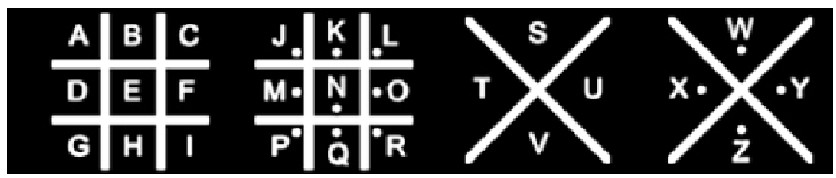
\includegraphics{1.jpg}
\end{center}

Then use the part of the table next to this letter to replace it when encrypting.\\

So if the plaintext is: code, the ciphertext is:\\

Summarizing the previous classic classical encryption algorithms, it can be found that whether it is single-table encryption or multi-table encryption, it is based on two ideas, one is substitution and the other is shifting. The so-called substitution or replacement refers to the use of another symbol to replace the characters in the plain text, and the movement is to exchange the order of the characters in the plain text to achieve the purpose of confusion. Most of the previous algorithms use the idea of ​​substitution, while one type of encryption algorithm uses the idea of ​​shifting. For example, the fence encryption algorithm, its basic idea is to write the plaintext along the diagonal, while reading the ciphertext line by line, for example, for the plaintext: I AM A GOOD STUDENT.\\

\begin{center}
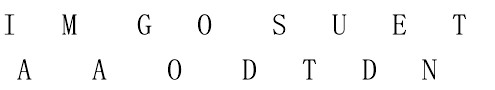
\includegraphics{2.jpg}
\end{center}

The cipher text is: IMGOSUETAAODTDN. The encryption algorithm invented by Sparta in ancient Greece is based on the idea of ​​shifting. The characters in the cipher text are the characters in the plain text, but the order is disturbed.\\


\section{Conclusion}


The confidentiality of many algorithms in classical encryption algorithms is based on the confidentiality of the algorithm itself, which is different from modern encryption algorithms. It is precisely because the algorithm itself is kept secret, it is not conducive to the development of cryptography. The development of cryptography in the stage of classical cryptography is very slow.


\section{Reference}


[1].信息安全小百科  密码学发展史[J].保密科学技术,2014(03):73.\par
[2].邓勇进.古典密码学[J].硅谷,2011(07):14.

\end{document}



